\section{Theoretical explanation}

\subsection{Signal Model}

\begin{frame}
  \frametitle{Signal Model}
  \begin{itemize}
    \item In our model, we assume a training sequence (preamble) is known to the receiver (DA operation). 
    \item The goal is to estimate accurately the start time of the preamble and to estimate carrier phase and frequency offsets from the preamble. 
    \item The received samples $r_p$ are given by
\begin{equation}
    \begin{aligned}
      \label{eq:model}
      r_p = s_{p-\bar{p}}Ae^{j\phi}e^{j2\pi\delta p}+w_{p},
    \end{aligned}
  \end{equation}
where
\begin{itemize}
    \item $p$ is the global time axis measuring the position of samples in the entire received stream.
    \item $\bar{p}$ denotes the start position of the received preamble.
    \item $s_n$ is the pulse-shaped preamble for $n=0,1,\ldots,N-1$.
    \item $\xi=Ae^{j\phi}$, $\delta$ are the unknown phasor and frequency offsets.
    \item $w_p$ is complex AWGN.
\end{itemize}
\end{itemize}
  
\end{frame}

\subsection{Time Synchronization}

\begin{frame}
    \frametitle{Time synchronization}

    \begin{center}
      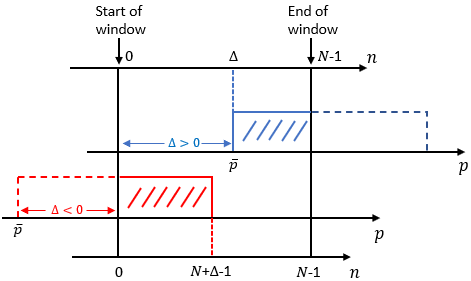
\includegraphics[width=.38\textwidth]{partial_preamble_detection.png}
    \end{center}

    \begin{itemize}
      \item Two hypotheses for sequential detection task are given by:
      
      \begin{equation}
        \label{eq:two hypotheses}
        \begin{aligned}
        &H_0{:}~r_n{=}
        \begin{dcases}
            s_{n-\Delta}\xi e^{j2\pi\delta (n-\Delta)}{+}w_n & \max(0{,}\Delta){\leq} n {<} \min(N{,}N{+}\Delta) \\
            w_n & \text{otherwise},
        \end{dcases} \\
        &H_1{:}~r_n{=}s_n\xi e^{j2\pi\delta n}+w_n,
        \end{aligned}
      \end{equation}
      where
      
      \begin{itemize}
          % \item $H_0$: the received signal is the channel noise or only contains a portion of the preamble.
          % \item $H_1$: the received signal contains the entire preamble.
          \item $\Delta$ is the distance between the current start position of the observation window and the true position of the preamble $\bar{p}$.
      \end{itemize}

    \end{itemize} 

\end{frame}


\begin{frame}
    \frametitle{Hypothesis Testing}
    \begin{itemize}

      \item The conditional likelihood ratio test (CLRT) is built by conditioning on $\Delta$, the phasor $\xi$, and the frequency offset $\delta$
  
      \begin{equation}
          \label{eq:log likelihood}
          \begin{aligned}
          \Re\Bigg\{\sum_{n=0}^{N-1}r_ns_n^*\xi^*e^{-j2\pi\delta n}-\sum_{n=\Delta}^{N-1}r_n&s_{n-\Delta}^*\xi^*e^{-j2\pi\delta(n-\Delta)}\Bigg\} \LRT{H_1}{H_0} \\
          &\frac{N_0}{2}\ln\eta+\frac{A^2}{2}\sum_{n=N-\Delta}^{N-1}|s_n|^2.
          \end{aligned}
      \end{equation}
  
      \begin{itemize}
          \item The two inner products on left hand side are the matched filters for hypothesis $H_1$ and $H_0$.
          \item The matched filter for $H_0$ is not computable in practice due to the unknown information of $\Delta$.
          \item The effect of the partial correlation can be neglected by using a preamble with very good autocorrelation property.
      \end{itemize}
      
  \end{itemize}

\end{frame}

\begin{frame}
  \frametitle{The Sequential Detector}
    \begin{itemize}
    
        \item A practical sequential detector is given based on the above discussion for each observation window at global sample index $p$
        \begin{equation}
          \label{eq:generalized_corr}
          \rho(p)=
          \frac{\Re\{\langle
            \boldsymbol{r}_{p},\hat{\boldsymbol{s}}_{p}\rangle\}}
          {||\boldsymbol{r}_{p}||\cdot||\hat{\boldsymbol{s}}_{p}||} \LRT{H_1}{H_0} \gamma
        \end{equation}

        where 
        \begin{itemize}
          \item $\bm{r}_{p}{=}[r_{p},r_{p+1},\ldots,r_{p+N-1}]$ denotes the received signal in the observation window
          starting at position $p$.
          \item $\hat{\bm{s}}_{p}$ denotes the carrier-corrected preamble,
          where each element is $\hat{s}_{n}=s_n\hat{\xi}_{p}e^{j2\pi\hat{\delta}_{p}n}$
          for $n=0,1,\ldots,N{-}1$, and $\hat{\xi}_{p}$, $\hat{\delta}_{p}$ are the carrier estimates at
          position $p$.
          \item A realistic generalized likelihood ratio test (GLRT) replaces the CLRT.
          \item The complexity of estimating $\hat{\xi}$,$\hat{\delta}$ is critical for practical implementation. 

        \end{itemize}
        
        
    \end{itemize}

\end{frame}

\subsection{Carrier Synchronization}

\begin{frame}
  \frametitle{Carrier Synchronization}
    \begin{itemize}
    
       \item Assume that the time synchronization is perfect.
       \item The maximum likelihood estimation (MLE) of the parameters in the signal model is given by
       
       \begin{equation}
        \label{eq:ML_f_xi}
        \hat{\delta},\hat{\xi}=\min_{\delta,\xi=Ae^{j\phi}}\sum_{n=0}^{N-1}|r_n-s_n\xi e^{j2\pi\delta n}|^{2}.
      \end{equation}

      \item The closed form for $\hat{\xi}$ and a necessary condition for $\hat{\delta}$ are obtained by taking the Wirtinger derivative
      
      \begin{equation}
        \label{eq:opt_xi}
        \hat{\xi}=\frac{\sum_{n=0}^{N-1}{r_{n}s_n^{*}e^{-j2\pi\hat{\delta} n}}}{\sum_{n=0}^{N-1}|s_{n}|^2},
      \end{equation}

      \begin{equation}
        \label{eq:necessary condition for delta}
        J(\hat{\delta}) = \Im\bigg\{\sum_{k=1}^{N-1}{\sum_{m=k}^{N-1}{kr_{m-k}r_m^{*}s_{m-k}^{*}s_m}e^{j2\pi\hat{\delta}k}}\bigg\}=0.
      \end{equation}

    \end{itemize}


\end{frame}


\begin{frame}
  \frametitle{Coarse Estimator: Single-Lag Estimator with Partial Coherent Integration}

    \begin{itemize}
    
      \item At moderate SNR, every lag $k$ can be used to approximate the frequency estimate $\delta$. This suggests that an unbiased estimate of $\delta$ can be obtained by using only a single lag $k$.
      \item To extend the operation to low SNR, a generalized SL estimator with PCI is derived
      
      \begin{equation}
        \label{eq:single_lag_estimator_w_partial_corr}
        \hat{\delta}_{SL}^{(v)}(k_v)=-\frac{\arg\big\{\sum_{l=k_v}^{N/v-1}\digamma_l^{*(v)}\digamma_{l-k_v}^{(v)}\big\}}{2\pi k_vv},
      \end{equation}

      where $\digamma_{l}^{(v)}$ is the result of PCI over block $l$
      of length $v$

      \begin{equation}
        \label{eq:coherent_integrator}
        \digamma_l^{(v)}=\sum_{n=lv}^{(l+1)v-1}r_ns_n^*, \quad \text{for}~l=0,1,\ldots,N/v{-}1.
      \end{equation}

      \begin{itemize}
        \item  $k_v=\lfloor k/v \rfloor$.
      \end{itemize}

    \end{itemize}

    % \begin{center}
    %   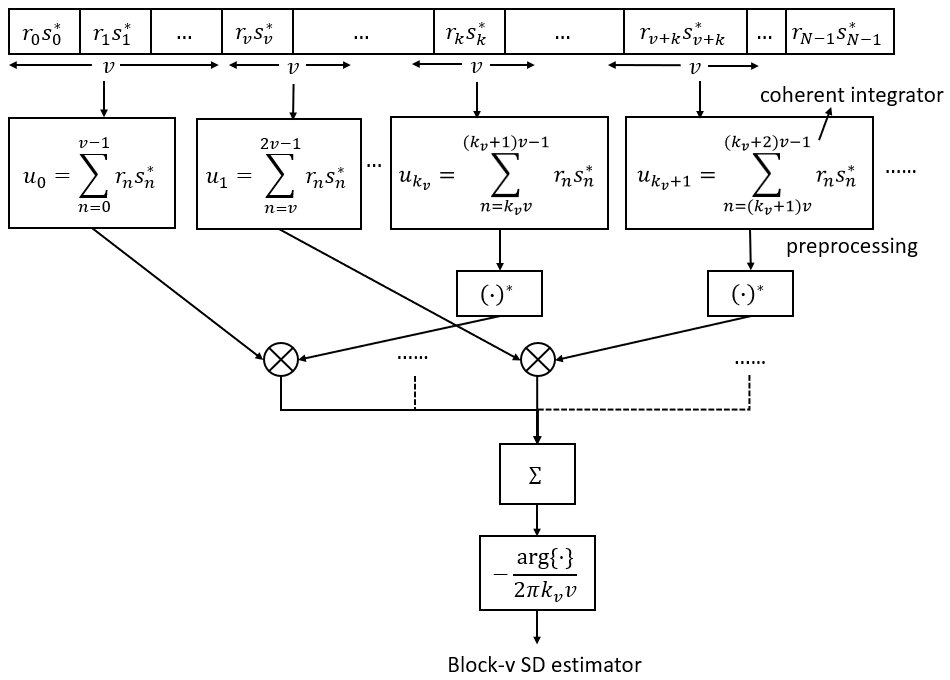
\includegraphics[width=.5\textwidth]{general_SD_estimator.png}
    % \end{center}


\end{frame}



\begin{frame}
  \frametitle{Block diagram}

    \begin{center}
      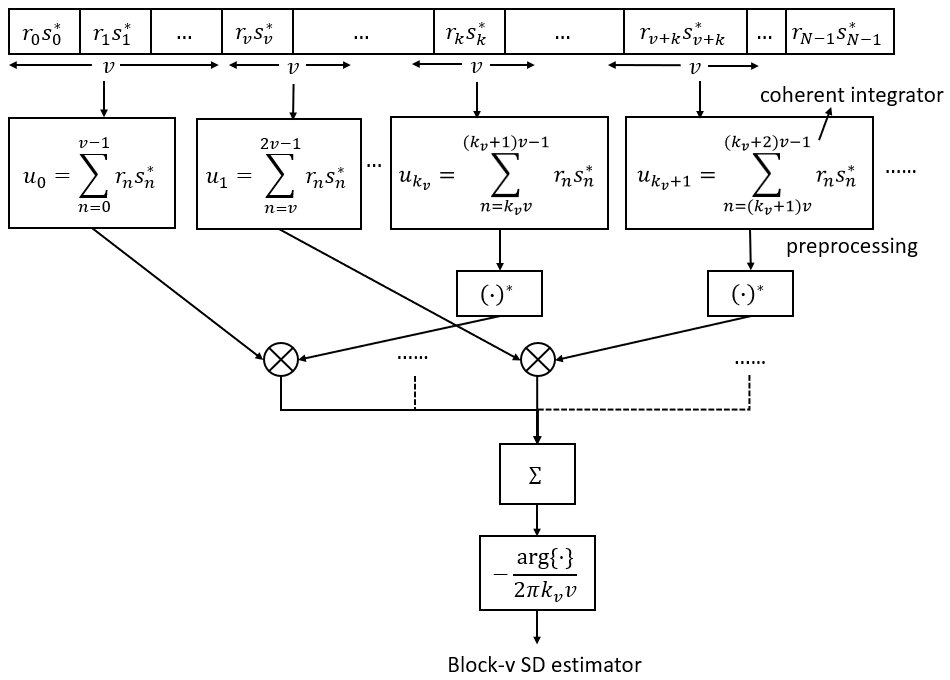
\includegraphics[width=.5\textwidth]{general_SD_estimator.png}
    \end{center}

    \begin{itemize}
    
      \item The above figure illustrates how Single-Lag estimator with PCI works.
      \item The intention of PCI is to increase the SNR of coherent terms before estimating frequency offset from non-coherent terms by leveraging the processing gain.
      \item The complexity is degraded by $O(N)$.

    \end{itemize}

    % \begin{center}
    %   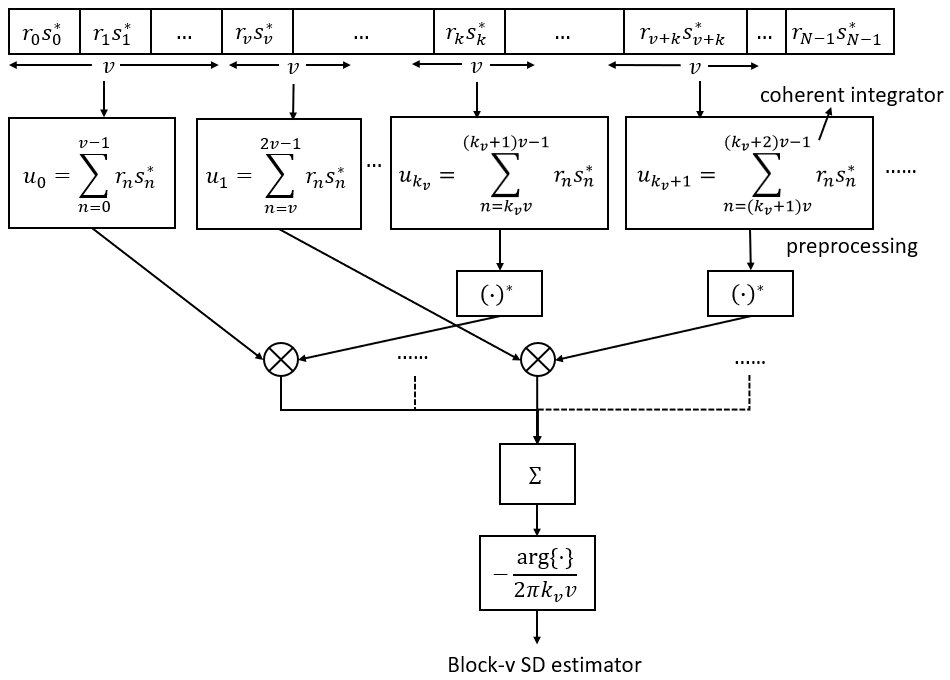
\includegraphics[width=.5\textwidth]{general_SD_estimator.png}
    % \end{center}


\end{frame}


\begin{frame}
  \frametitle{Probability distribution over non-coherent blocks}

    \begin{itemize}
    
      \item Define $C_{\digamma}(v,l)=\digamma_l^*\digamma_{l-k_v}$ and it has a mixed distribution of a complex Gaussian and 
      a Bessel function of the second kind (from noise), whose mean and variance are

      \begin{equation}
        \begin{aligned}
        \label{eq:mean_var_product_coherent_int}
        \mu_{C_{\digamma}}&=\frac{E_s}{M}\sum_{n=lv}^{(l+1)v-1}e^{-j2\pi \delta n}\bigg(\sum_{m=(l-k_v)v}^{(l-k_v+1)v-1}e^{j2\pi \delta m}\bigg) \\
        &=E_s/M\cdot e^{-j2\pi \delta k_vv}\D^2(v,\delta), \\
        \sigma^2_{C_{\digamma}}&={\underbrace{N_0^2v^2/4}_{\text{from Bessel}}}+{\underbrace{N_0E_sv/M\cdot\D^2(v,\delta)}_{\text{from Complex Gaussian}}},
        \end{aligned}
      \end{equation}

      where 
      \begin{itemize}
        \item $\D(v,\delta) = \frac{\sin(\pi \delta v)}{\sin(\pi
        \delta)}$ is the Dirichlet function of $\delta$, which approaches 
        the maximum value $v$ at $\delta=0$.
      \end{itemize}


    \end{itemize}

    % \begin{center}
    %   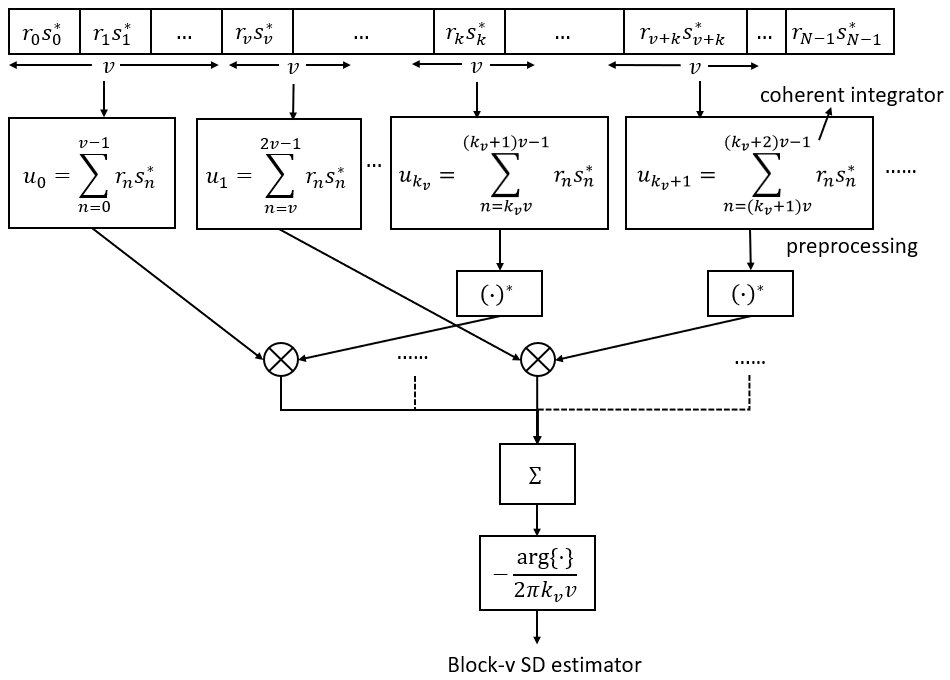
\includegraphics[width=.5\textwidth]{general_SD_estimator.png}
    % \end{center}


\end{frame}


\begin{frame}
  \frametitle{Performance improvement by PCI}

    \begin{itemize}

      \item One way to look at the performance of the SL estimator with PCI is by the "output" SNR
      
      \begin{equation}
        \begin{aligned}
          \label{eq:SNR_out}
          \text{SNR}_{\sum C_{\digamma}}^{(v,\delta)}=\frac{|\mu_{\sum C_{\digamma}}|^2}{\sigma^2_{\sum C_{\digamma}}} 
          =\frac{(N/v-k_v)\cdot\D^4(v,\delta)}
          {v^2/\text{SNR}_{\text{in}}+2v\cdot\D^2(v,\delta)}\cdot\text{SNR}_{\text{in}}. \\
        \end{aligned}
      \end{equation}
    
      \begin{itemize}
        \item The "output" SNR is degraded by the variance of the second kind Bessel random variable.
      \end{itemize}

      \item To see PCI improves the performance of SL at low SNR via the ratio
      
      \begin{equation}
        \begin{aligned}
          \label{eq:relative_processing_gain}
          \frac{\text{SNR}_{\sum C_{\digamma}}^{(v,0)}}{\text{SNR}_{\sum C_{\digamma}}^{(1,0)}}
          \approx\frac{v+2v\cdot\text{SNR}_{\text{in}}}{1+2v\cdot\text{SNR}_{\text{in}}}.
        \end{aligned}
      \end{equation}

      \begin{itemize}
        \item the relative performance increases with $v$ at very low SNR.
      \end{itemize}

    \end{itemize}

    % \begin{center}
    %   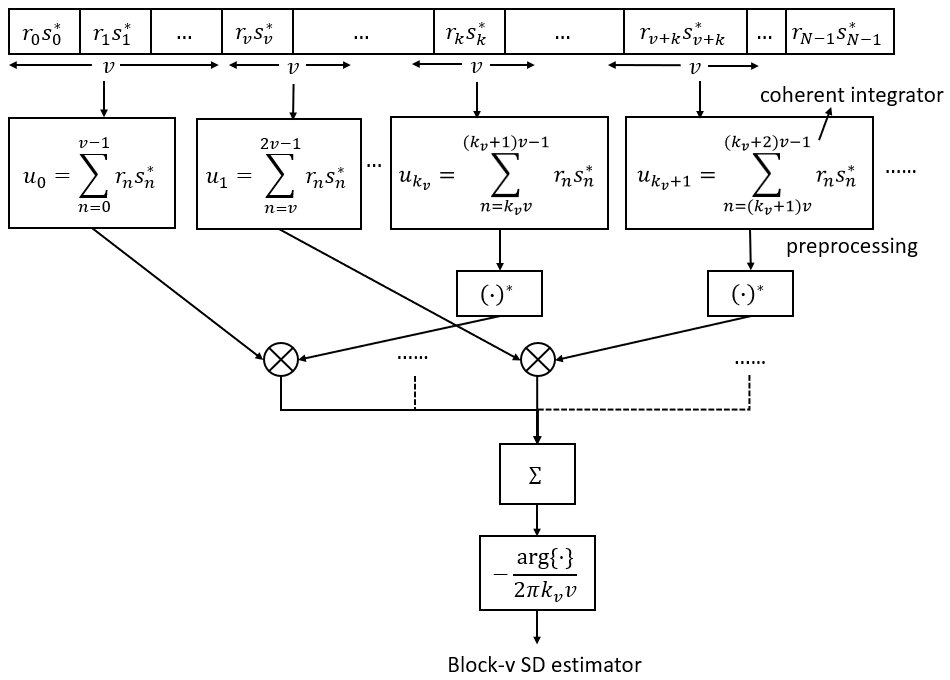
\includegraphics[width=.5\textwidth]{general_SD_estimator.png}
    % \end{center}


\end{frame}


\begin{frame}
  \frametitle{Fine Estimator: Newton-Method based Estimator}

    \begin{itemize}
    
      \item Use the SL estimator as starting point for a Newton-type iteration aimed at finding a better solution to the necessary condition for $\hat{\delta}$ in~\eqref{eq:necessary condition for delta}
      
      \begin{equation}
        \label{eq:iter_NM_est}
        \hat{\delta}_{NM}^{(i+1)}=\hat{\delta}_{NM}^{(i)}-
        \frac{J(\hat{\delta}_{NM}^{(i)})}{J^\prime(\hat{\delta}_{NM}^{(i)})}
      \end{equation}

      \begin{itemize}
        \item $\hat{\delta}_{NM}^{(0)}=\hat{\delta}^{(v)}_{SL}(k_v)$.
        \item $J^\prime(\cdot)$ is the derivative of $J$ with respect to $\hat{\delta}$.
        \item A single iteration is usually sufficient to achieve very good accuracy.
        \item Complexity is $O(N^2)$.
      \end{itemize}

      \item Summary: The SL estimator is used for operating at high sample rate for sequential detection task due to its low complexity.
      The NM estimator improves the accuracy after reliable detection to enable coherent demodualtion.
        

    \end{itemize}




\end{frame}

\subsection{Simulation}

\begin{frame}
  \frametitle{Simulation Results}

    \begin{center}
      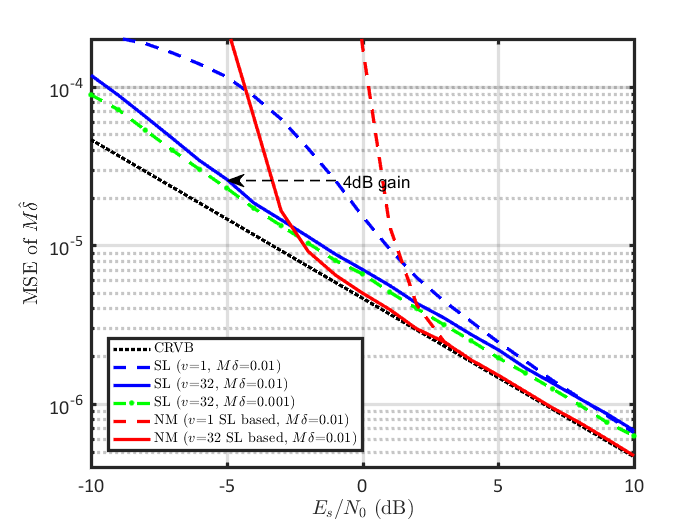
\includegraphics[width=.521\textwidth]{accuracy_NM_SL_slides.png}
    \end{center}

    \begin{itemize}
    
      \item The accuracy is improved from SL w/o PCI at $\SI{-1}{\dB}$ to with PCI at $\SI{-5}{\dB}$ by $\SI{4}{\dB}$ gain, which is consistent with~\eqref{eq:relative_processing_gain}.
      \item The accuracy of SL is higher at all SNRs with lower frequency offset because of the Derichlet function.  
      \item NM approaches the CRVB as SL reaches some accuracy.

    \end{itemize}




\end{frame}

\begin{frame}
  \frametitle{Simulation Results}

    \begin{center}
      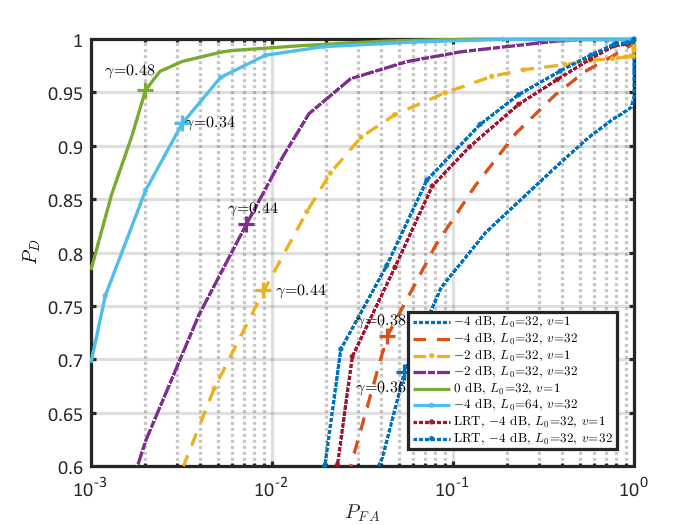
\includegraphics[width=.521\textwidth]{ROC_new.png}
    \end{center}

    \begin{itemize}
    
      \item The above figure shows the receiver operating characteristics (ROC) of the sequential detector.
      \item The better accuracy of SL with PCI also improves the detection performance at low SNR.
      \item The performance can also be significantly improved by leveraging a larger size of the preamble.

    \end{itemize}

\end{frame}